\documentclass[a4paper,12pt]{article}


% % % % % % % % % % % % % % % % % % % % % % % % % % % % %
% % ATTENTION : dans les figures le label doit être mis 
%APRES le caption pour que le numéro de la figure lorqu'on
%la référence soit le bon ; sinon on a le numéro du paragraphe
% % % % % % % % % % % % % % % % % % % % % % % % % % % % %

% package qui fournit \justify 
\usepackage[document]{ragged2e}

%pifont pour les puces de formes spéciales
\usepackage{pifont}
\usepackage[table]{xcolor}
\usepackage{tabu}
% césure exemple
% \hyphenation{an-ti-cons-ti-tu-tion-nel

\usepackage[utf8x]{inputenc}
\usepackage[T1]{fontenc}
\usepackage[frenchb]{babel} % If you write in French
%\usepackage[english]{babel} % If you write in English
\usepackage{lmodern} % Pour changer le pack de police
\renewcommand*\familydefault{\sfdefault}
\usepackage{makeidx}
\usepackage{amsthm}
\usepackage{amsmath}
\usepackage{amssymb}
\usepackage{mathrsfs}
\usepackage{stmaryrd}
\usepackage{geometry}
%\usepackage{graphicx}
\usepackage{graphbox}
\usepackage{supertabular}
\usepackage{tabularx}
\usepackage{longtable}
\usepackage{pdflscape}
\geometry{hmargin=2cm,vmargin=2cm}

\usepackage{booktabs}
\usepackage{tabularx}
\usepackage[table]{xcolor}
\usepackage{ltablex}
\usepackage{float}
\usepackage{url}

\usepackage{chngcntr}
\counterwithin*{footnote}{page}


\usepackage[titletoc,toc,title,page]{appendix}
\renewcommand{\appendixtocname}{Annexes}
\renewcommand{\appendixpagename}{Annexes}

\usepackage{standalone}
\usepackage{ifthen}
\usepackage{xstring}
\usepackage{calc}
\usepackage{pgfopts}
\usepackage{tikz}
\usetikzlibrary{positioning,shapes,shadows,arrows}
%\usepackage{array,ragged2e}
\usepackage{algpseudocode}
\usepackage{algorithm}
\makeatletter
\renewcommand{\ALG@name}{Algorithme}
\renewcommand{\listalgorithmname}{Table des algorithmes}

\newtheorem{theo}{Définition}[section]
\usepackage{mathtools, bm}
\usepackage{amssymb, bm}

\usepackage{hyperref}
\hypersetup{
    colorlinks=true,       % false: boxed links; true: colored links
    linkcolor=black,       % color of internal links
    citecolor=purple,       % color of links to bibliography
    urlcolor=blue          % color of external links
}

\usepackage{listings}

\definecolor{dkgreen}{rgb}{0,.6,0}
\definecolor{dkblue}{rgb}{0,0,.6}
\definecolor{dkyellow}{cmyk}{0,0,.8,.3}

\lstset{
  language        = php,
  basicstyle      = \small\ttfamily,
  keywordstyle    = \color{dkblue},
  stringstyle     = \color{red},
  identifierstyle = \color{dkgreen},
  commentstyle    = \color{gray},
  emph            =[1]{php},
  emphstyle       =[1]\color{black},
  emph            =[2]{if,and,or,else},
  emphstyle       =[2]\color{dkyellow}}



\usepackage{blindtext}
\usepackage{enumitem} % pour changer les puces dans \itemize


\date{\today}

\makeindex
\def\siecle#1{\textsc{\romannumeral #1}\textsuperscript{e}}
\newcommand{\argmax}{\mathop{\mathrm{argmax}}\nolimits}
\newcommand{\pgcd}{\mathop{\mathrm{pgcd}}\nolimits}

\makeatletter
\renewcommand{\pod}[1]{\allowbreak\mathchoice
  {\if@display \mkern 18mu\else \mkern 8mu\fi (#1)}
  {\if@display \mkern 18mu\else \mkern 8mu\fi (#1)}
  {\mkern4mu(#1)}
  {\mkern4mu(#1)}
}

\usepackage{wallpaper}
%\usepackage{bsymb,b2latex}
\begin{document}
\renewcommand{\labelitemi}{\textbullet}
% pour factoriser l'échelle des figures 
%utilisation scale=\scaledvwa au lieu de scale = 0.3 ... 
\newcommand{\scaledvwa}{0.4} 
\newcommand{\scaledvw}{0.3}
\newcommand{\scalekad}{0.45}


\phantomsection
\begin{titlepage}
	\parindent=0pt
\ThisTileWallPaper{1.3\paperwidth}{1.0\paperheight}{images/ctrl2}
 
\addtolength{\wpXoffset}{-4.5cm}

%	\vspace*{\stretch{1}}
%	\begin{center}
%		\includegraphics[scale=0.5]{images/enac.png}%
%	\end{center}
	
\color{white}{	\vspace*{\stretch{1}} }
	\hrulefill
	\begin{center}\bfseries\Huge
		\color{white}
		{Méthode formelle de conception : Système de contrôle du trafic aéroportuaire} 
	\end{center}
	\hrulefill
	
	\vspace*{1cm}
	\begin{center}\bfseries\Large
			\color{white}
		{Jules HELLER - Abdelkader BELDJILALI}
		
	\end{center}
	
	\vspace*{\stretch{2}}


\end{titlepage}
%on créé la couverture

\pagebreak

\tableofcontents
\justify

\pagebreak

\section*{Introduction}
\addcontentsline{toc}{section}{Introduction}

intro ...








\section{Généralités}

Le système est modélisé sous forme d'une machine à états-transitions. Les états sont caractérisés par des constantes respectant des axiomes et des variables respectant des conditions nommées "invariants". Les constantes caractérisent le "contexte" du système i.e. l'aspect statique. Les variables décrivent l'aspect dynamique. Les transitions sont désignées par le terme event. Les events sont des actions conditionnées ou non par une garde. Une garde est une condition qui autorisera ou non l'action du système. La transition du système est supposée instantanée et se produire dès que la garde est vraie. Il peut survenir des cas d'indéterminisme externe lorsque plusieurs gardes sont vraies simultanément. Si elles sont toutes fausses, le système est bloqué. Si, à tout instant, une garde est vraie, le système ne se termine jamais.

\paragraph{}
La démarche itérative proposée dans l'exercice consiste à écrire les exigences a partir des spécifications ; chaque exigence est identifiée par un label qui permet la traçabilité et le classement en catégories notamment fonctionnelle et environnementale. On part d'un modèle abstrait simple, formalisé dans l'outil rodin. Des preuves notamment d'invariance sont effectuées. Le plugin Atelier B génère des obligations de preuves dans un langage correspondant à la logique du premier ordre associée à la théorie des ensembles.Atelier B utilise notamment une base de règles d’inférence associée à un moteur contenant des heuristiques et un prouveur de type SAT.

\paragraph{} Le modèle formel est corrigé le cas échéant par ajout de gardes ou de conditions sur les gardes si on cherche à éviter les blocages. Les exigences sont complétées si nécessaire. Enfin par raffinement successifs, on passe d'une vision synoptique du système à une vue plus détaillée qui peut conduire jusqu'à la phase d'implémentation.


\section{Expression textuelle des exigences}


%\subsection{}
%\paragraph{}

\subsection{Description du système et de son environnement}
\begin{figure}[H]
	\begin{center}	
		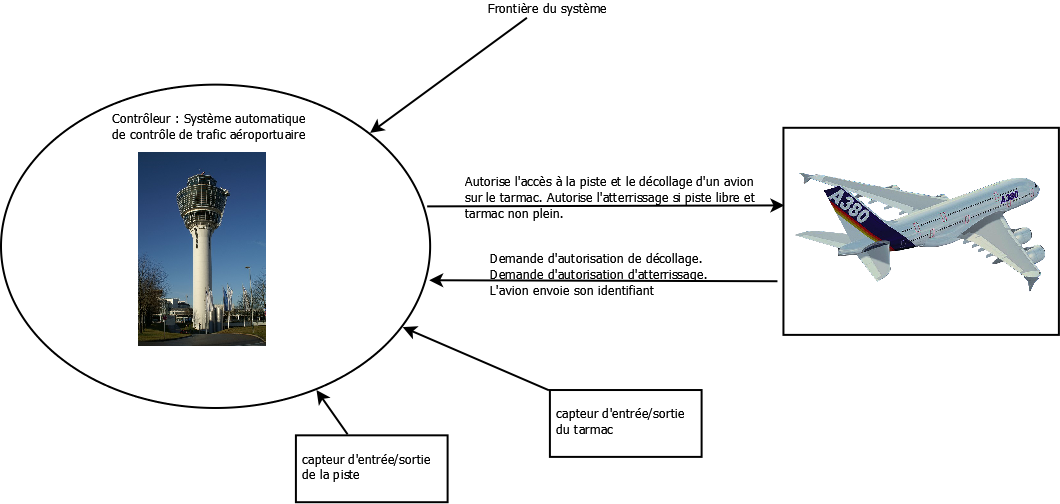
\includegraphics[scale=0.3]{images/ctx}
		\caption{Environnement du système}
		\label{ctx}
	\end{center}
\end{figure}


\subsection{Analyse des spécifications}

\paragraph{}

Le système à concevoir est un \textbf{contrôleur aérien automatique} chargé de contrôler le trafic sur le tarmac et d'autoriser l'accès à la piste des avions prêts au décollage. 
\paragraph{}
Ce système est un logiciel qu'on appelera le Contrôleur. Ce contrôleur interagit avec son environnement à savoir les pilotes et des capteurs non précisés dans l'énoncé. Les spécifications sont incomplètes car le contrôleur doit forcément autoriser ou refuser les avions à l'atterrissage également. Il est nécessaire d'avoir un capteur qui permet de compter les avions qui entrent et sortent du tarmac et un autre capteur qui assure le comptage des avions sur la piste. Les avions ne peuvent atterrir que si l'aéroport n'est pas plein, 20 places maximum sont disponibles. 
\paragraph{}
On suppose que les clearances sont données aux avions qui se trouvent sur le tarmac. Dès l'autorisation de décoller donnée, l'avion se rend sur la piste et décolle. Il n'y a pas d'étape intermédiaire. Un système de communication sécurisé de type data-link doit exister pour donner les clearances et recevoir les identifiants et les demandes des pilotes.

\paragraph{}
On suppose qu'il ne peut y avoir qu'un seul avion sur la piste ; pas de possibilité
de mettre deux avions au décollage en même temps.


\subsection{Reformulation des exigences}

\begin{table} [H]
	
	\centering
\rowcolors{2}{gray!65}{white}
\begin{tabu}{|[2pt] p{1.7cm} | [2pt]p{15cm}|[2pt]}

	\tabucline[2pt]{-} \rowcolor{yellow}
\Centering	\textbf{Label}& \Centering \textbf{Exigence}  \\ \tabucline[2pt]{-}

	\hline 
	FON-1&Le contrôleur doit autoriser les avions à décoller et atterrir  \\ 
	\hline 
FON-2	& Le nombre d'avions immobilisés sur le tarmac est limité à 20 y compris ceux en attente de décollage \\ 
	\hline 
	FON-3& Des avions entrent et quittent la piste d'atterrissage décollage  \\ 
	\hline 
	FON-4& Des avions entrent sur le tarmac et le quittent  \\ 
	\hline 
	FON-5& La piste ne peut être occupée par un avion au décollage et un avion à l'atterrissage en même temps. \\ 
	\hline 
	FON-6& Le nombre de décollages ou atterrissages successifs n'est pas limité   \\ 
	\hline 
	FON-7& Le contrôleur doit fixer et délivrer les clearances à l'avance   \\ 
	\hline 
	FON-8& Le contrôleur ne doit autoriser l'avion qu'après l'envoi de son identifiant    \\ 
		\hline
	FON-9& Le contrôleur doit soit refuser, soit accepter, soit mettre en attente l'avion demandeur   \\ 
 	\hline
 FON-10& Le contrôleur doit refuser la clearance après 10mn de mise en attente.   \\ 
	\hline 
   ENV-1 &Tout avion se dirigeant vers la piste doit avoir une autorisation de décoller \\ 
   	\hline 
   ENV-2 &Le système est muni d'un capteur qui permet de compter les avions sur la piste \\ 
   \hline 
   ENV-3 &Le système est muni d'un capteur qui permet de compter les avions sur la tarmac \\ 
\tabucline[2pt]{-}
\end{tabu} 
\caption{Tableau des exigences V1}
\end{table}


\section{Première modélisation abstraite}
	
%\subsection{}
%\paragraph{}

   On veut initialement considérer très peu d'exigences. L'énoncé nous indique
   que seules les entrées et sorties de l'espace de l'aéroport sont étudiées. On effectue donc une étude formelle sur un système très simplifié où la piste et le tarmac ne sont pas pris en compte. Nous étudions uniquement les échanges d'avions entre l'espace de l'aéroport et l'espace extérieur ce qu'on modélise en utilisant deux events ou transitions :
   
   \begin{itemize}
   	\item extout lorsqu'un avion sort de l'espace extérieur pour rentrer dans l'espace aéroportuaire,
   	\item extin lorsqu'un avion entre dans l'espace extérieur.
   \end{itemize} 

\begin{figure}[H]
	\begin{center}	
		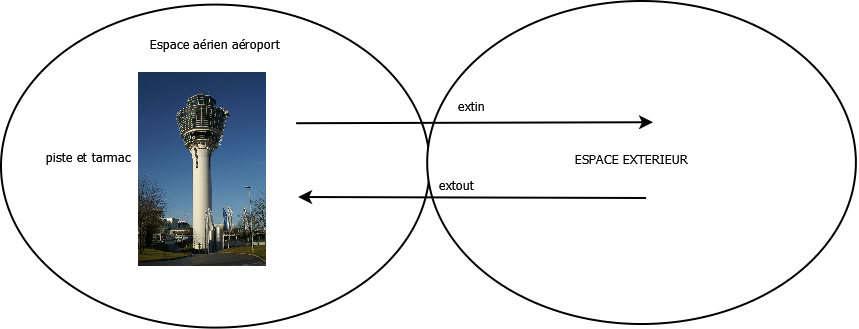
\includegraphics[scale=0.4]{images/mod0}
		\caption{Modèle abstrait}
		\label{mod0}
	\end{center}
\end{figure}

On fait abstraction de la piste. Ainsi, la seule variable à considérer est le nombre total d'avions présents dans l'espace de l'aéroport à un instant donné. On note nt cette variable.

\paragraph{Etat static ou \textit{contexte} du système :}
L'état statique est caractérisé par ntmax, le nombre total maximum d'avions dans  l'espace de l'aéroport i.e. la capacité de l'aéroport:
\begin{figure}[H]
	\begin{center}	
		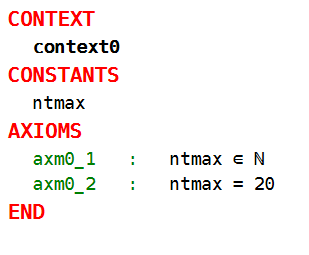
\includegraphics[scale=0.8]{images/ctx0}
		\caption{Etat static du système}
		\label{ctx0}
	\end{center}
\end{figure}

\paragraph{Etat dynamique du système :}
 L'état dynamique du système n'est constitué que de cette seule variable. Elle est définie au moyen de deux conditions ou \textit{invariants} :
%   \begin{align}
%  inv0\_1 : nt \in ℕ 
%   \end{align}
%   
%    \begin{align}
%   inv0\_2 : nt \le ntmax
%   \end{align}
%   

\begin{figure}[H]
	\begin{center}	
		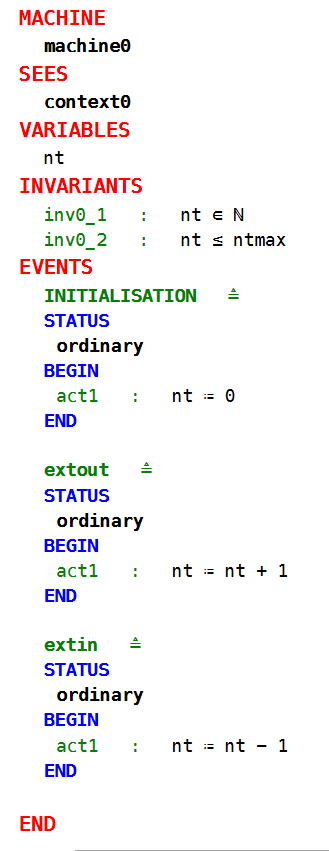
\includegraphics[scale=0.8]{images/mac0}
		\caption{Etat dynamique du système}
		\label{mac0}
	\end{center}
\end{figure}

\begin{figure}[H]
	\begin{center}	
		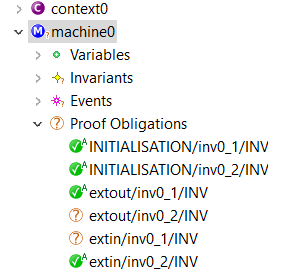
\includegraphics[scale=0.8]{images/proof1}
		\caption{Echec de deux preuves obligatoires}
		\label{proof1}
	\end{center}
\end{figure}

\begin{figure}[H]
	\begin{center}	
		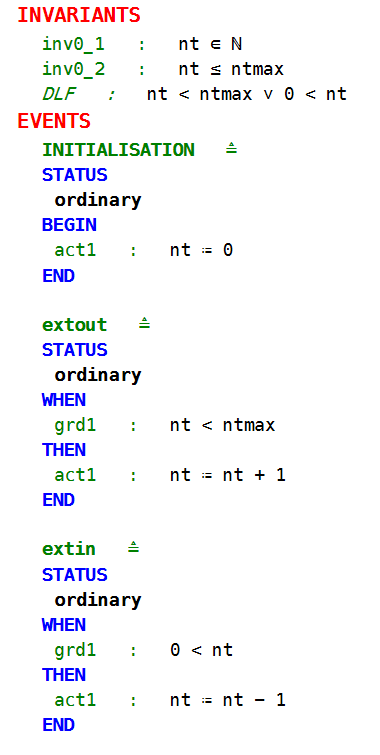
\includegraphics[scale=0.8]{images/garde}
		\caption{Ajout de 2 gardes et d'un théorème pour éviter les blocages}
		\label{garde}
	\end{center}
\end{figure}

\paragraph{conclusion}
Pour débuguer le modèle formel initial, il a fallu ajouter deux gardes pour garantir un nombre d'avions compris entre 0 et 20 et éviter les deadlock. Les exigences sont mises à jour pour tenir compte de ces oublis.

\begin{table} [H]
	
	\centering
	\rowcolors{2}{gray!65}{white}
	\begin{tabu}{|[2pt] p{1.7cm} | [2pt]p{15cm}|[2pt]}
		
		\tabucline[2pt]{-} \rowcolor{yellow}
		\Centering	\textbf{Label}& \Centering \textbf{Exigence}  \\ \tabucline[2pt]{-}
		
		\hline 
		FON-1&Le contrôleur doit autoriser les avions à décoller et atterrir  \\ 
		\hline 
		FON-1.1& \textcolor{red}{Le contrôleur doit fonctionner indéfiniment une fois lancé.}  \\ 
		\hline 
		FON-2	& Le nombre d'avions immobilisés sur le tarmac est limité à 20 y compris ceux en attente de décollage\textcolor{red}{mais doit rester positif} \\ 
		\hline 
		FON-3& Des avions entrent sur et quittent la piste d'atterrissage décollage  \\ 
		\hline 
		FON-4& Des avions entrent sur le tarmac et le quittent  \\ 
		\hline 
		FON-5& La piste ne peut être occupée par un avion au décollage et un avion à l'atterrissage en même temps. \\ 
		\hline 
		FON-6& Le nombre de décollages ou atterrissages successifs n'est pas limité   \\ 
		\hline 
		FON-7& Le contrôleur doit fixer et délivrer les clearances à l'avance   \\ 
		\hline 
		FON-8& Le contrôleur ne doit autoriser l'avion qu'après l'envoi de son identifiant    \\ 
		\hline
		FON-9& Le contrôleur doit soit refuser, soit accepter, soit mettre en attente l'avion demandeur   \\ 
		\hline
		FON-10& Le contrôleur doit refuser la clearance après 10mn de mise en attente.   \\ 
		\hline 
		ENV-1 &Tout avion se dirigeant vers la piste doit avoir une autorisation de décoller \\ 
		\hline 
		ENV-2 &Le système est muni d'un capteur qui permet de compter les avions sur la piste \\ 
		\hline 
		ENV-3 &Le système est muni d'un capteur qui permet de compter les avions sur la tarmac \\ 
		\tabucline[2pt]{-}
	\end{tabu} 
	\caption{Tableau des exigences V2}
\end{table}

\section{Premier raffinement}

\subsection{Analyse}
Dans cette partie, on introduit la piste pour évoluer vers un modèle plus concret. On peut ainsi spécifier le nombre d'avions se trouvant sur la piste en vue  d'un décollage et après un atterrissage ainsi que le nombre d'avions sur le tarmac.
Ce fait implique un "raffinement" des exigences environnementales ; on doit avoir un capteur capable de compter les avions au décollage et un capteur pour les avions à l'atterrissage. Ce qui donne les exigences modifiées suivantes :


\begin{table} [H]
	\centering
\rowcolors{2}{gray!65}{white}
\begin{tabu}{|[2pt] p{1.7cm} | [2pt]p{15cm}|[2pt]}
	
	\tabucline[2pt]{-} \rowcolor{yellow}
	\Centering	\textbf{Label}& \Centering \textbf{Exigence}  \\ \tabucline[2pt]{-}
	
	\hline 
	FON-1&Le contrôleur doit autoriser les avions à décoller et atterrir  \\ 
	\hline 
	FON-1.1& \textcolor{red}{Le contrôleur doit fonctionner indéfiniment une fois lancé.}  \\ 
	\hline 
	FON-2	& Le nombre d'avions immobilisés sur le tarmac est limité à 20 y compris ceux en attente de décollage\textcolor{red}{mais doit rester positif} \\ 
	\hline 
	FON-3& Des avions entrent sur et quittent la piste d'atterrissage décollage  \\ 
	\hline 
	FON-4& Des avions entrent sur le tarmac et le quittent  \\ 
	\hline 
	FON-5& La piste ne peut être occupée par un avion au décollage et un avion à l'atterrissage en même temps. \\ 
	\hline 
	FON-6& Le nombre de décollages ou atterrissages successifs n'est pas limité   \\ 
	\hline 
	FON-7& Le contrôleur doit fixer et délivrer les clearances à l'avance   \\ 
	\hline 
	FON-8& Le contrôleur ne doit autoriser l'avion qu'après l'envoi de son identifiant    \\ 
	\hline
	FON-9& Le contrôleur doit soit refuser, soit accepter, soit mettre en attente l'avion demandeur   \\ 
	\hline
	FON-10& Le contrôleur doit refuser la clearance après 10mn de mise en attente.   \\ 
	\hline 
	ENV-1 &Tout avion se dirigeant vers la piste doit avoir une autorisation de décoller \\ 
	\hline 
	ENV-2 &\textcolor{blue}{Le système est muni d'un capteur qui permet de compter les avions sur la piste à l'atterrissage et un capteur pour les avions sur la piste au décollage.} \\ 
	\hline 
	ENV-3 &Le système est muni d'un capteur qui permet de compter les avions sur la tarmac \\ 
	\tabucline[2pt]{-}
\end{tabu} 
\caption{Tableau des exigences V3}
\end{table}

\begin{figure}[H]
	\begin{center}	
		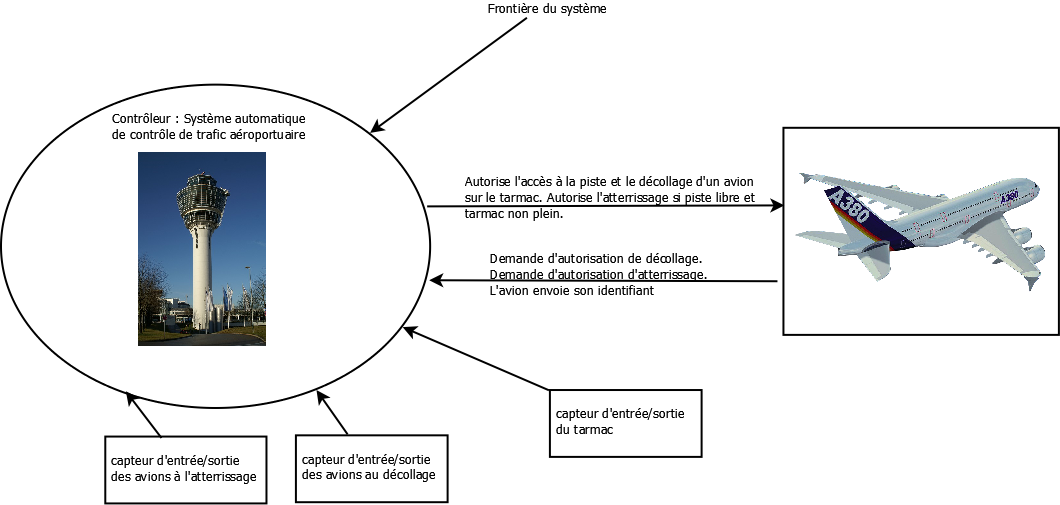
\includegraphics[scale=0.3]{images/1/env2}
		\caption{Environnement du système : version 2}
		\label{ctx}
	\end{center}
\end{figure}
\begin{figure}[H]
	\begin{center}	
		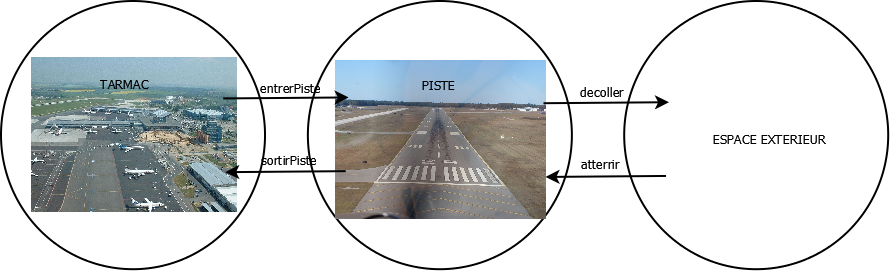
\includegraphics[scale=0.4]{images/1/raf1}
		\caption{Premier raffinement du système : piste et tarmac sont différenciés}
		\label{raf1}
	\end{center}
\end{figure}
\paragraph{}
Contrairement à ce qui se passe dans la réalité, les spécifications laissent la possibilité d'avoir au même moment plusieurs avions sur la piste au décollage ou à l'atterrissage dès lors qu'on ne mélange pas les décollages et atterrissages.
La piste est, à un instant donné, en sens unique.


%\subsection{raffinement de l'état du système clos}
%\begin{figure}[H]
%	\begin{center}	
%		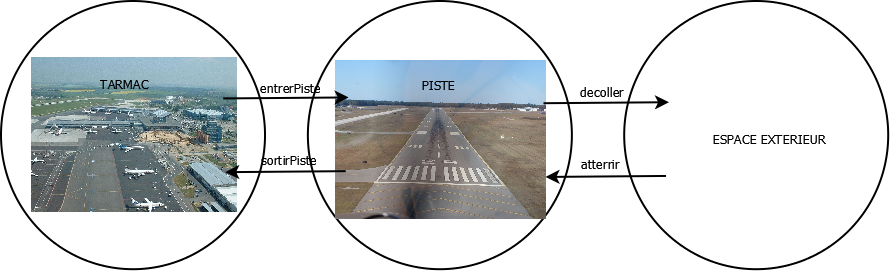
\includegraphics[scale=0.4]{images/1/raf1}
%		\caption{Premier raffinement du système : la piste et le tarmac sont différenciés}
%		\label{raf1}
%	\end{center}
%\end{figure}

\subsection{Contexte}
Le CONTEXTE n'est pas modifié. La constante ntmax du système caractérise l'état statique du système concret associé à ce premier raffinement.

\begin{figure}[H]
	\begin{center}	
		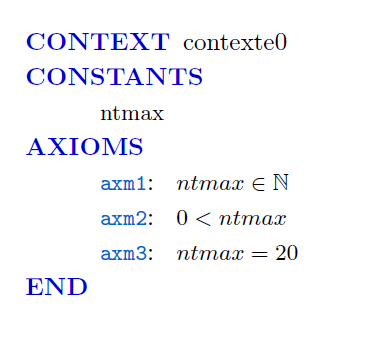
\includegraphics[scale=1]{images/1/ctx1}
		\caption{Contexte premier raffinement}
		\label{ctx1}
	\end{center}
\end{figure}

\subsection{Glue}Ces variables vérifient nbAvionsDecollage + nbAvionsAtterrissage + nbAvionsTarmac = nt. C'est l'invariant de "glue" qui fait le lien entre les 3 variables concrètes et la variable abstraite nt.

\subsection{Convergence des nouveaux events}

On définit un variant entier naturel, en l'occurrence, $nbAvionsTarmac + 2 ∗ nbAvionsAtterrissage$ dont on a vérifié qu'il est bien décrémenté par les deux nouveaux events introduits: $entrerPiste$ et $sortirPiste$ pour éviter qu'ils ne soient indéfiniment activés avec pour conséquence une interdition des décollages et atterrissages.

\subsection{Machine}
 On définit une nouvelle machine nommée "raffinement1" pour prendre en compte les nouvelles variables. La Machine raffinement1 est obtenue par raffinage de la machine0.
 \begin{figure}[H]
 	\begin{center}	
 		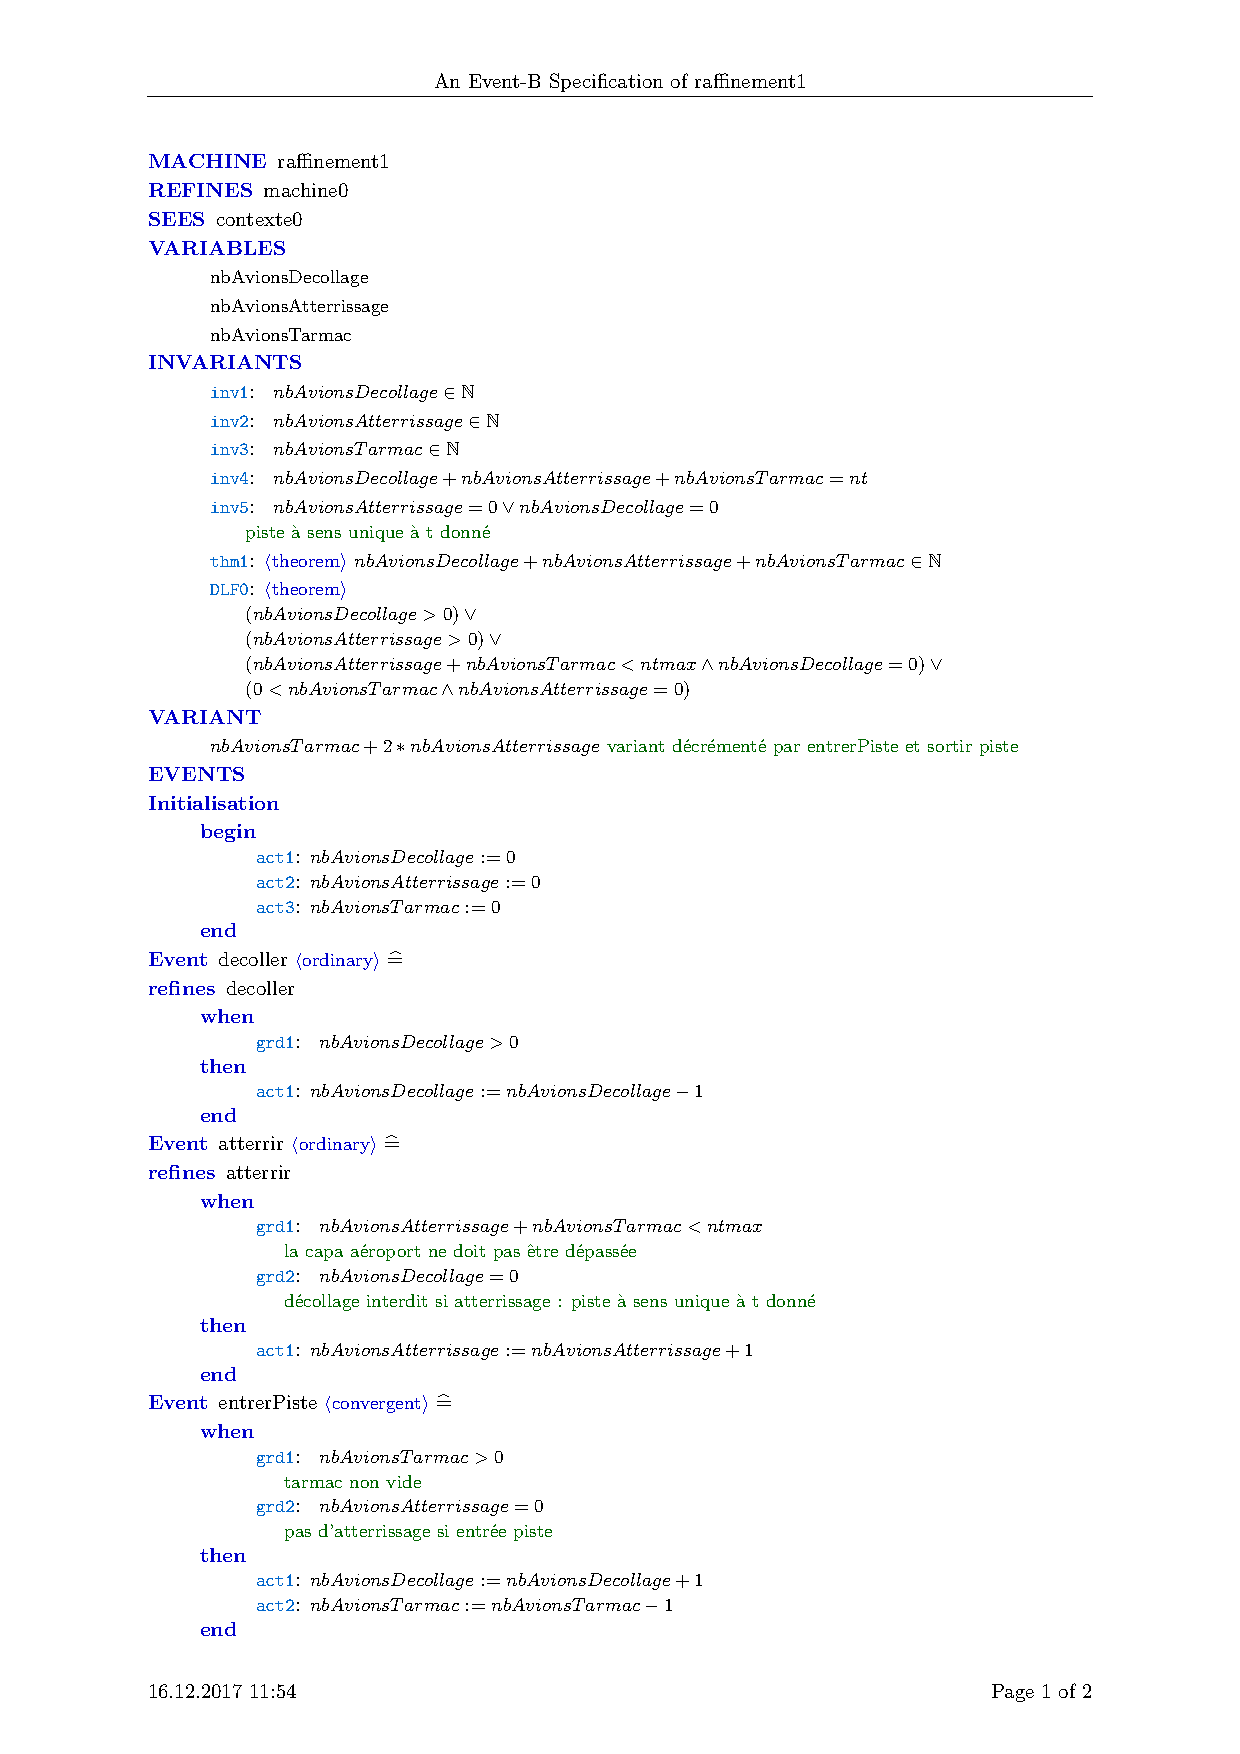
\includegraphics[scale=0.8]{images/1/machine1}
 		\caption{}
 		\label{machine1}
 	\end{center}
 \end{figure}
 
 \subsection{Preuves}
 
 Comme pour la machine abstraite, le théorème DLF0 doit être prouvé interactivement via la perspective "Proving" pour prendre en compte toutes les hypothèses.
 
 \begin{figure}[H]
 	\begin{center}	
 		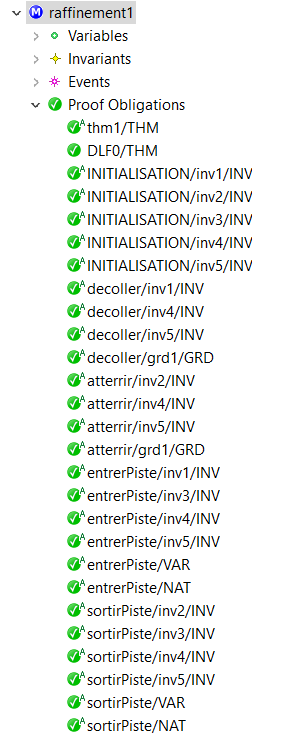
\includegraphics[scale=1.2]{images/1/proof1}
 		\caption{Preuves du premier raffinement}
 		\label{proof1}
 	\end{center}
 \end{figure}
 

 
 






\section{Second raffinement}


%\subsection{}
%\paragraph{}

\subsection{Analyse}
On introduit dans ce dernier raffinement les autorisations d'accès à la piste et les identifiants uniques à chaque avions. Un pilote effectue une demande d'accès
à la piste. Le système répond en accordant ou refusant le droit d'accès. 

\begin{itemize}
	\item Si l'accès est accordé, le pilote a 15 mn pour libérer la piste.
	\item S'il est refusé, le pilote doit attendre 5 mn avant de pouvoir renouveler sa demande.   
\end{itemize}  

\subsection{Contexte}
On étend le contexte0 précédent avec le contexte2

\begin{figure}[H]
	\begin{center}	
		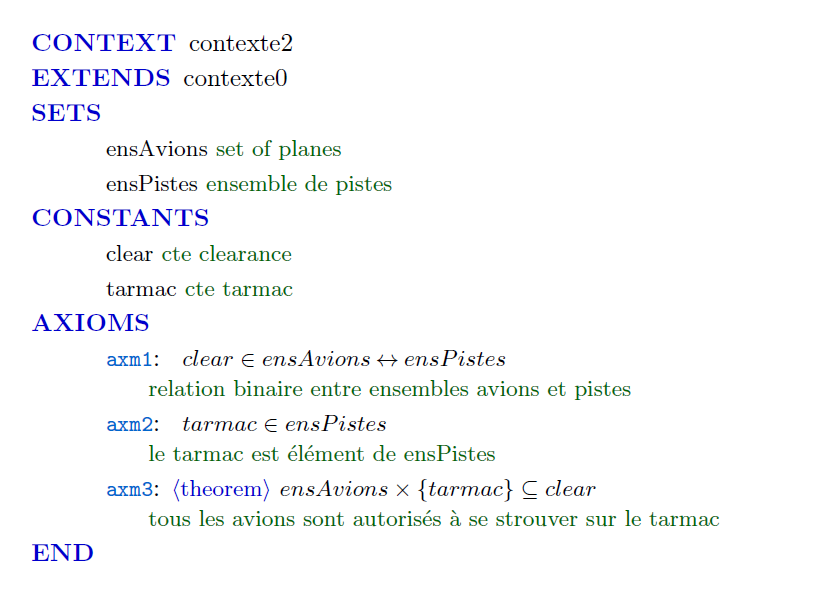
\includegraphics[scale=0.7]{images/2/ctx2}
		\caption{Contexte second raffinement}
		\label{ctx2}
	\end{center}
\end{figure}

\subsection{Glue} 
Le lien avec la machine raffinement1 est réalisé par le biais du nombre d'avions respectivement sur le tarmac, la piste décollage et la piste d'atterrissage. Une approche ensembliste, analogue à celle utilisée dans un système de contrôle d'accès à des bâtiments d'un site, conduit à introduire les ensembles d'avions correspondant. Les invariants de cardinalité, inv 16, 17 et 18 de la figure \ref{raf21} assure la liaison avec la machine parente. 


On crée une nouvelle machine nommée raffinement2 comme ci-après. Les commentaires ont été directement saisis dans l'interface rodin. Les livrables sont accessibles
en ligne via l'URI \url{https://github.com/kad15/eventb/tree/master/LIVRABLE_HELLER_BELDJILALI/workspace_rodin}.
\begin{figure}[H]
	\begin{center}	
		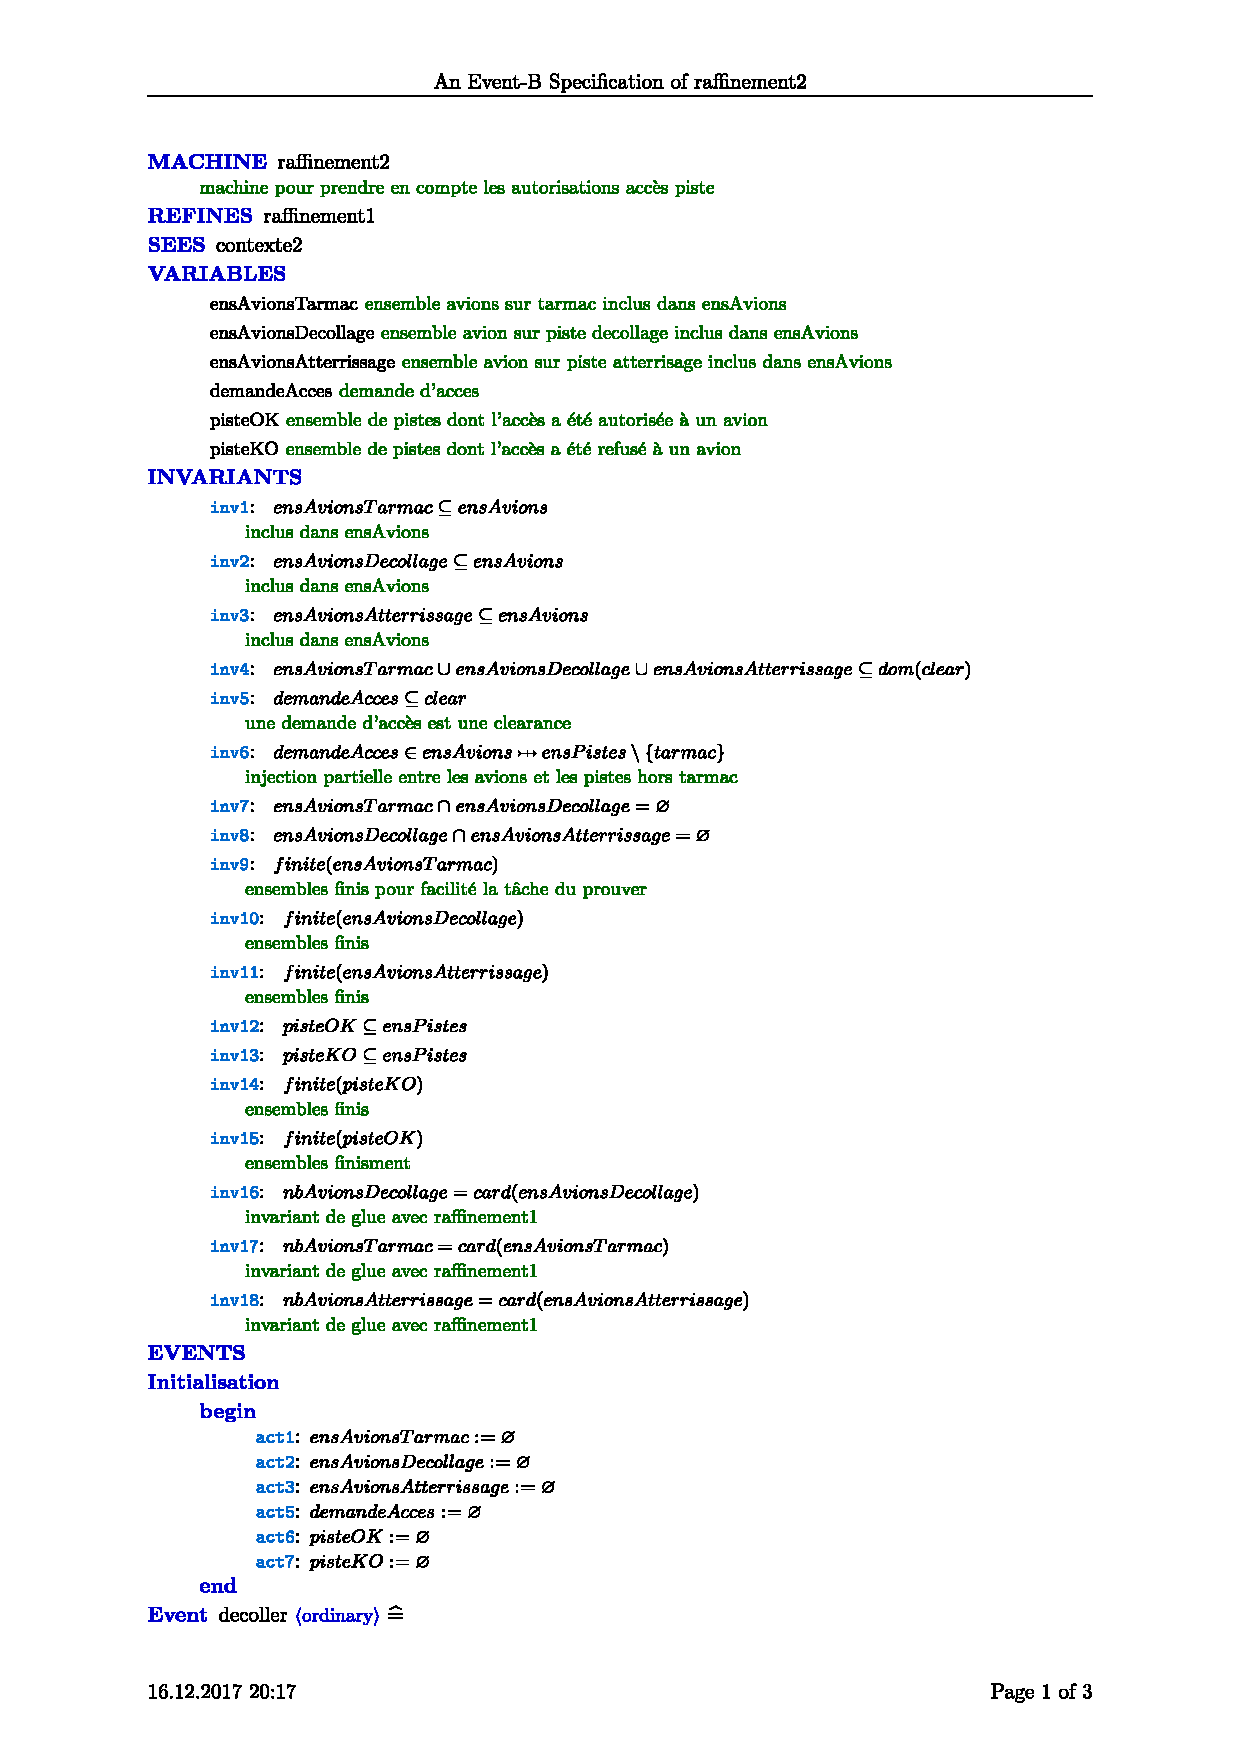
\includegraphics[scale=0.75]{images/2/raf21.pdf}
		\caption{ Machine : second raffinement}
		\label{raf21}
	\end{center}
\end{figure}

\begin{figure}[H]
	\begin{center}	
	
		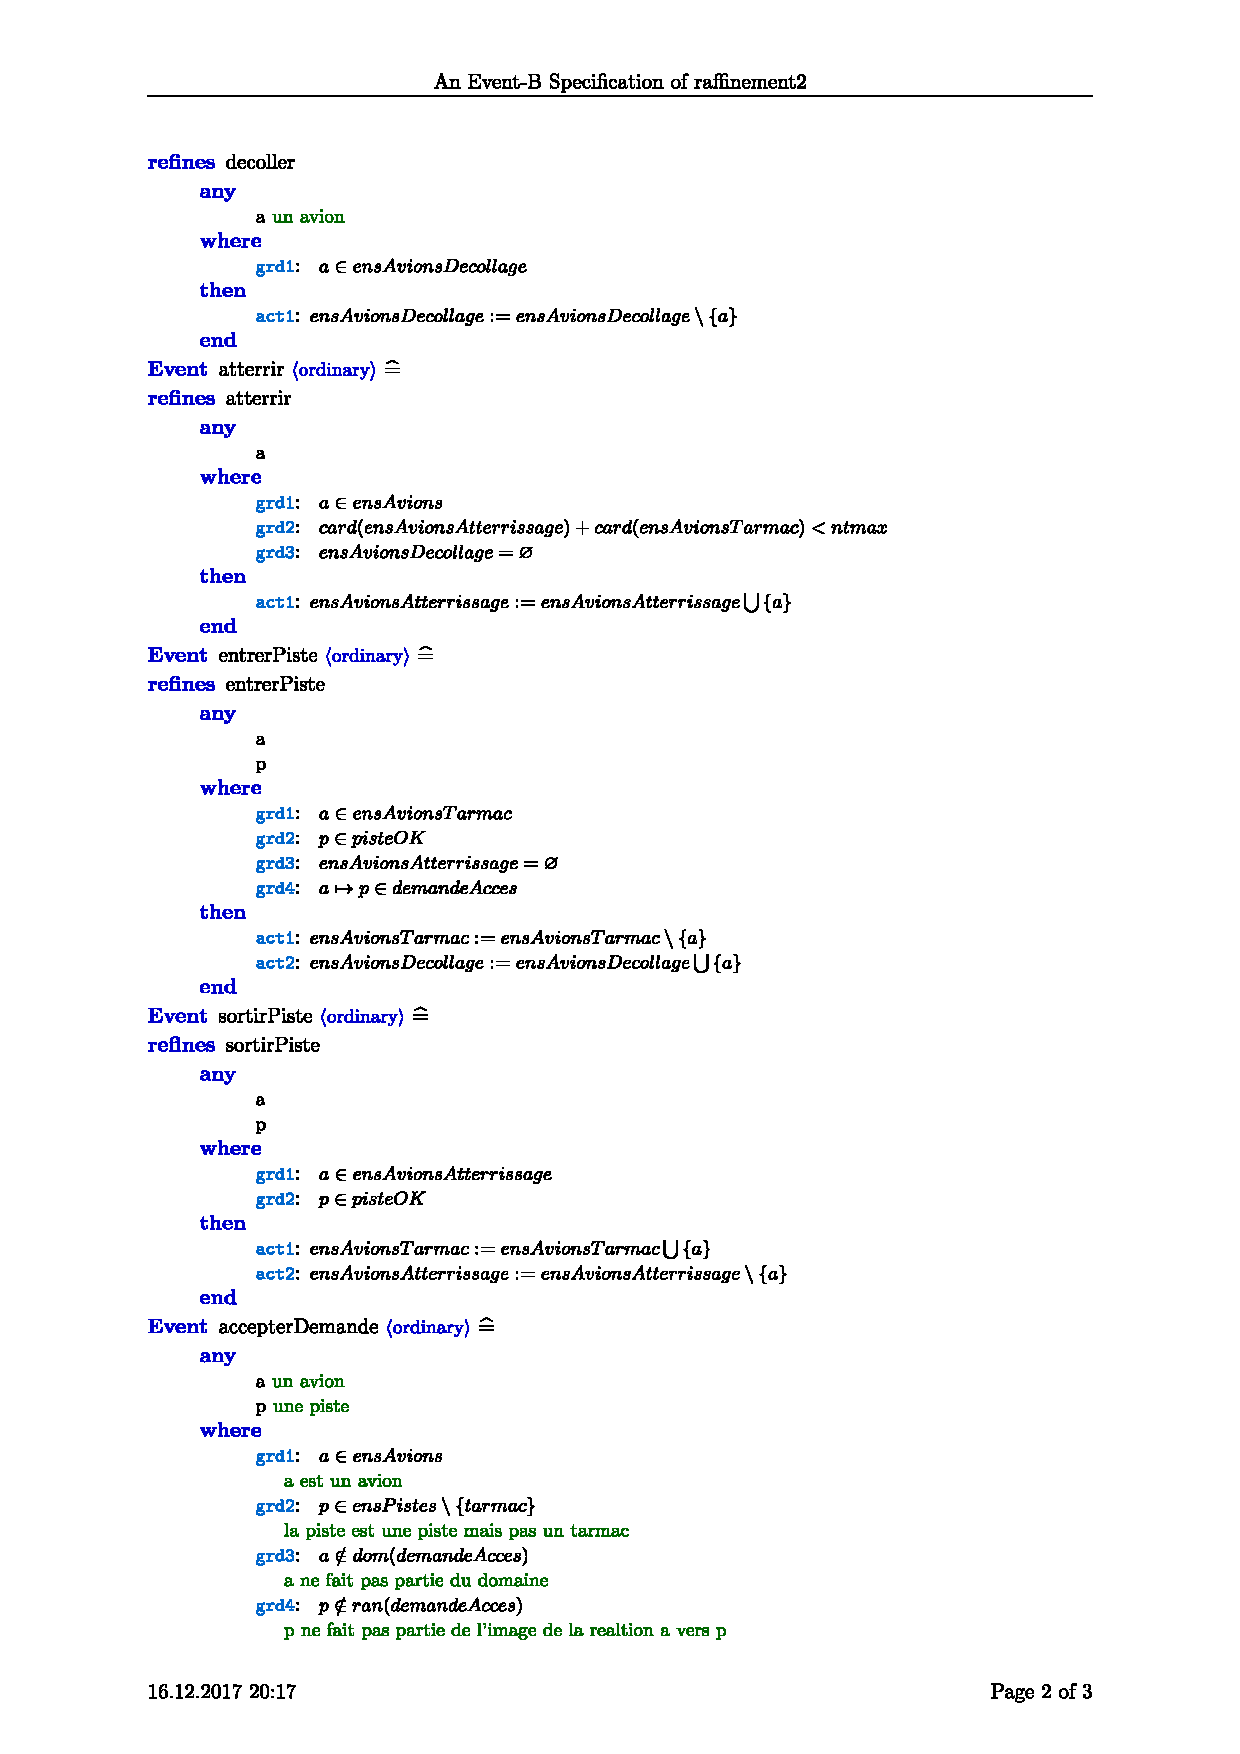
\includegraphics[scale=0.75]{images/2/raf22.pdf}
		\caption{ Machine : second raffinement (suite)}
		\label{raf22}
	\end{center}
\end{figure}


\begin{figure}[H]
	\begin{center}	
		
		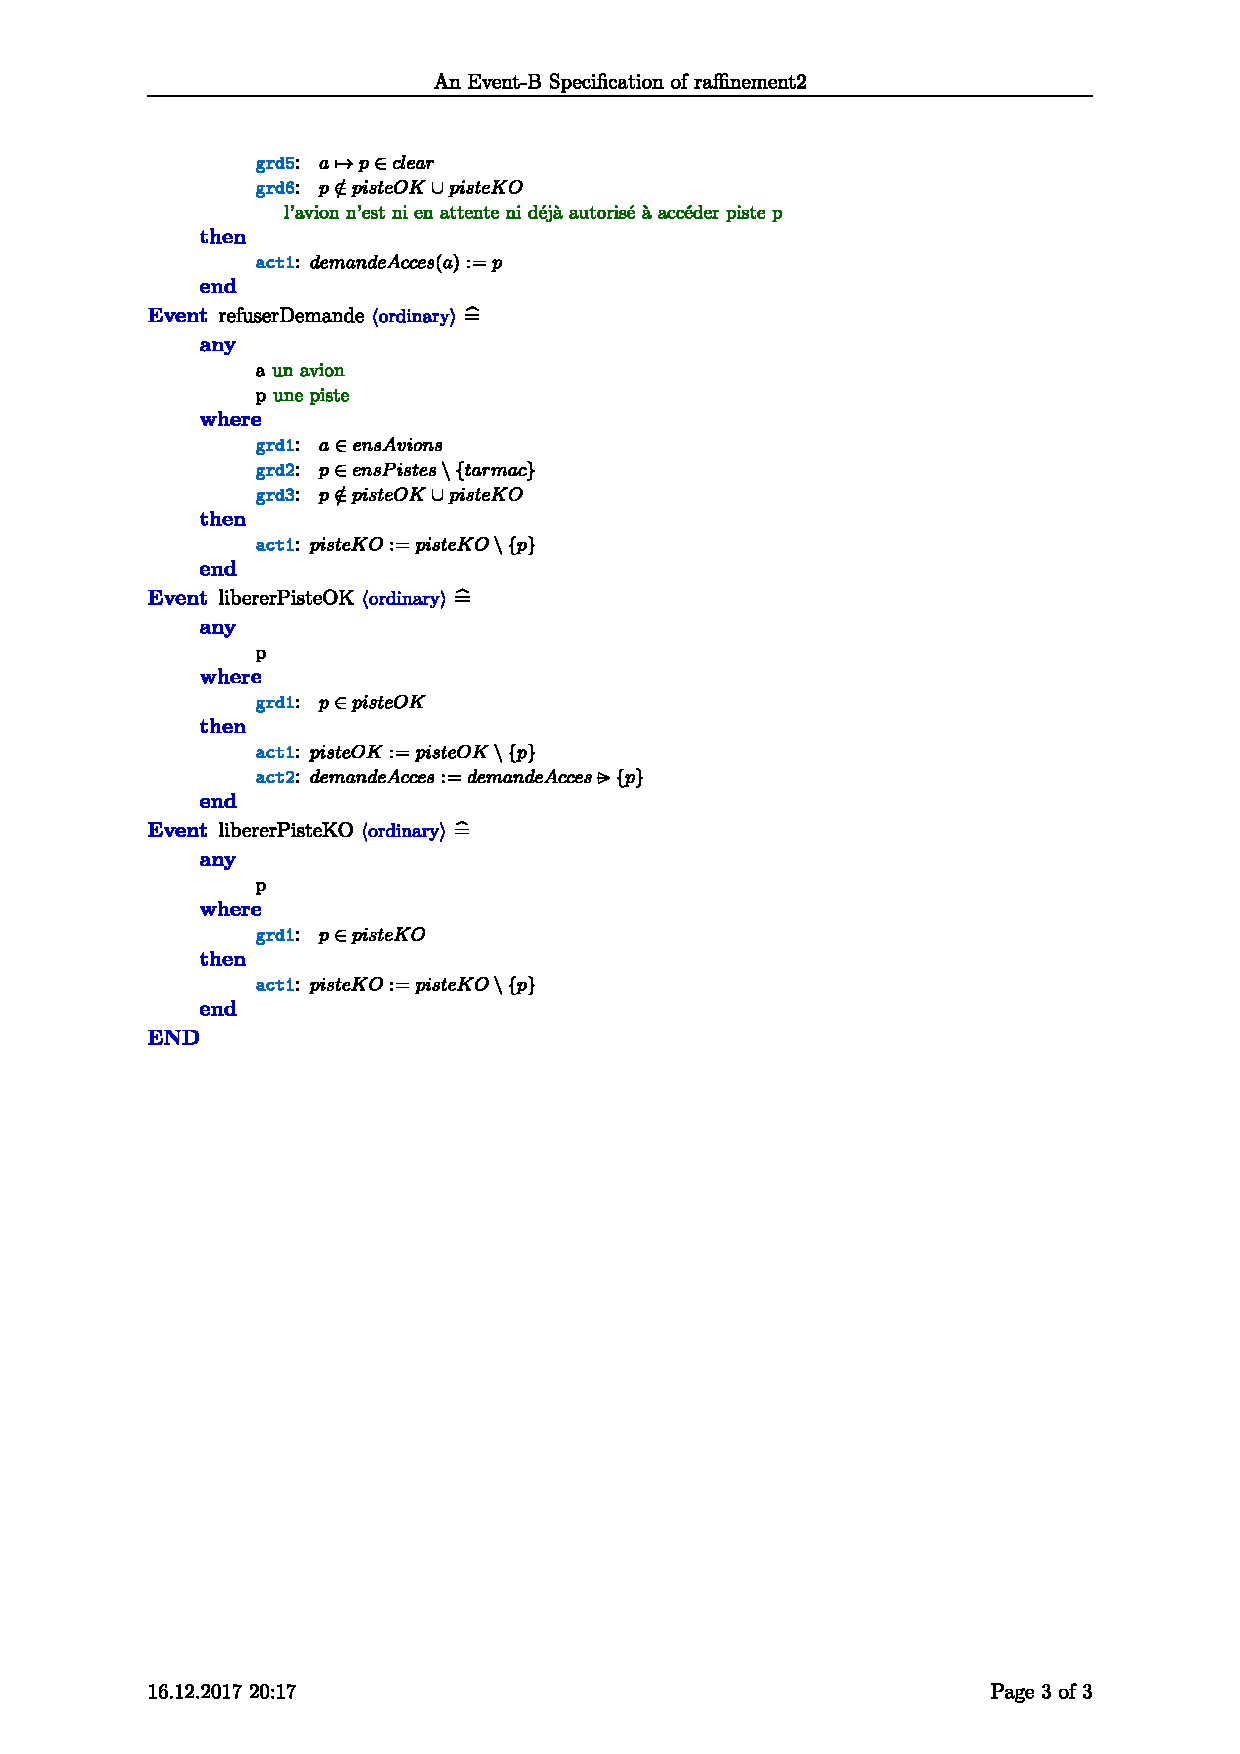
\includegraphics[scale=0.75]{images/2/raf23.pdf}
		\caption{ Machine : second raffinement (suite)}
		\label{raf23}
	\end{center}
\end{figure}


\subsection{Preuves}


\begin{figure}[H]
	\begin{center}	
		
		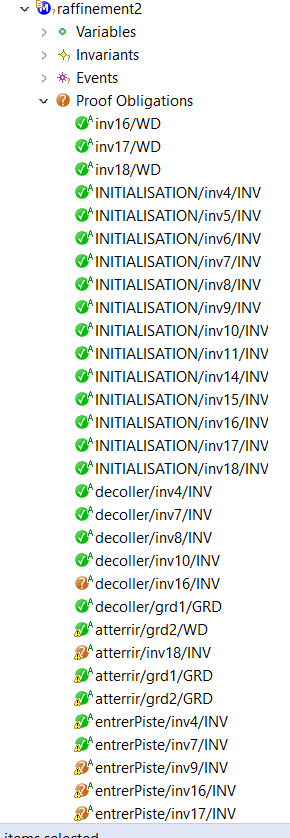
\includegraphics[scale=0.75]{images/2/proof2}
		\caption{ Résultat des preuves des propriétés générées par l'outil rodin - atelier B}
		\label{proof 2}
	\end{center}
\end{figure}

On constate que le système n'est pas entièrement validé. En outre, l'outil rodin indique une syntaxe incorrecte pour l'instruction $ensAvionsTarmac := ensAvionsTarmac ⋃ \{a\}$ alors qu'elle semble correcte.



\section*{Conclusion}
\addcontentsline{toc}{section}{Conclusion}

%Cette étude réalisée par raffinement successif montre qu’un système complexe peut être modélisé et validé de manière formelle grâce à des outils relativement simple. La difficulté dans l’implémentation se situe alors plutôt dans l’interprétation des exigences et dans la validation du modèle. Il est de plus important de montrer qu’un système entièrement modélisé et validé n’impose pas forcément un système totalement fonctionnel. En effet notre seconde machine était validée même avant d’avoir ajouté notre condition de non blocage. Il est alors très important de se poser des questions sur la viabilité du modèle réalisé et de bien vérifié que notre système ne peut se bloquer sur des événements limités.
%Finalement ce projet nous a montré l’importance de réaliser notre modélisation de manière successive, et donc par raffinement afin de pouvoir valider petit à petit notre modélisation sans être perdu dans quelque chose de trop complexe. La validation d’un modèle simple permet d’arriver plus confiant sur un modèle de plus haut niveau.
\paragraph{}



%\newpage
%\appendix
%\include{annexes/annexe_A}
%\include{annexes/annexe_B}

\newpage
\nocite{*}  %affiche toutes les entrées du bib même celles qui ne sont pas citées.
% cf.    http://www.tuteurs.ens.fr/logiciels/latex/bibtex.html
% compilation en TROIS PHASE  bibtex traite un fichier *.aux mais bibtex mon_fichier comme bibtex mon_fichier.aux sont acceptés 
% latex mon_fichier.tex
% bibtex mon_fichier
% latex mon_fichier.tex


% \renewcommand{\bibname}{Toto}
% ou
%\renewcommand{\refname}{Bibliographie}
% dans le préambule.
%\bibliographystyle{alpha}
%\bibliography{references}
\input{page-de-couverture/page_blanche}
\input{page-de-couverture/quatrieme-de-couv}
\end{document}
